\NewScheme{\SPOR}{SPOR}

\subsection{\Acfp*{SPOR}}%
\label{sec:global_overlay}
\label{sec:message_passing}

Say that Alice wants to send a message \(m\) to Bob.
Bob creates a reply header using \(\CreateReply\) and gives the output to Alice 
over an out-of-band channel.
We assume that \(m\) is either unavailable when the channel is used or too 
large to successfully send over the channel directly.
At a later point, Alice attaches a message \(m\) to the reply header using 
\(\UseReply\), creates a forward header using \(\CreateFwd\) with the prepared 
reply header as payload.
Then she sends this packet to the first node, which processes it using 
\(\ProcessHeader\).
The node will then process the header and in turn forward the packet to the 
next node.
At some point the message will reach Alice who identifies the message as the 
one expected to come from Bob.
(This process is illustrated in \cref{fig:file-exchange}.)
Now we will focus on how Alice and Bob choose the nodes that they provide to 
\(\CreateReply\) and \(\CreateFwd\).

\begin{figure}
  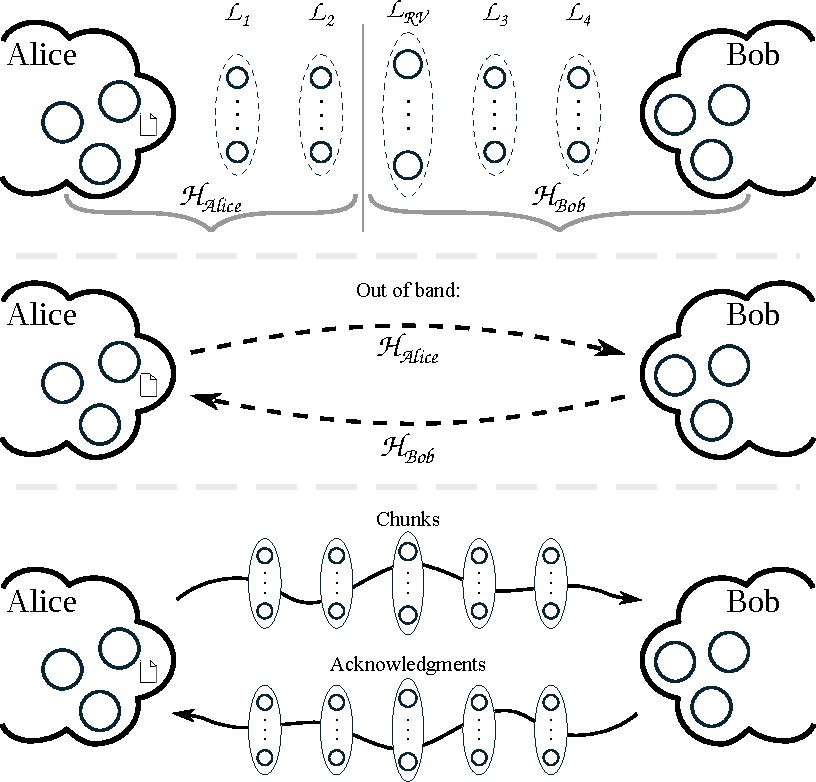
\includegraphics[width=\linewidth]{figures/file_exchange_v2.pdf}
  \caption{\label{fig:file-exchange}%
    A schematic of Alice and Bob sending a message using \name.
    \ding{1} illustrates the layer of the headers that Alice and Bob create.
    In \ding{2}, Alice and Bob exchange the headers out-of-band.
    In \ding{3}, Alice and Bob use two \ac{SPOR} routes, one for messages and 
    one for acknowledgements.
  }
\end{figure}

There are many uses of Sphinxes, many criteria that can be used to select the 
nodes in each layer.
We will focus on maximizing availability when routing in a network with high 
churn, but one could equally well select nodes to maximize, \eg, bandwidth.
We now describe a protocol, \ac{SPOR}, which uses Sphinxes to transfer messages 
from a source to a destination over a network of nodes with high churn.

\commentDaniel{We should describe how to do this selection using a prediction 
  oracle, then we provide a prediction oracle later.}
\commentDaniel{The stuff below is just as before, it must be edited.}

\newcommand{\viewsize}{\ensuremath{l_{\text{view}}\xspace}}
\newcommand{\view}{\ensuremath{\mathcal{V}_{\text{RPS}}\xspace}}
\NewAlgorithm{\GetRandomPeer}{\text{random descriptor from }\view}

To create PORs, devices need to know the address, encryption key, and probability of remaining available of some nodes in the system, to pick them as relays on the route.

To reach this goal, we employ Random Peer Sampling (RPS) \cite{Voulgaris_Gavidia_van_Steen_2005,Jelasity_Voulgaris_Guerraoui_Kermarrec_van_Steen_2007}.
Essentially, each node maintains a view \view containing \viewsize other devices' descriptors. 
This view is periodically updated as follows: a device $d$ pops the oldest descriptor $d'$ from its view, then swaps a predefined number of $l$ elements from \view with $d'$.
Both devices add a descriptor for themselves to the view exchange.
If $d'$ was offline, its descriptor is simply removed from the $d$'s view, but \view is otherwise not updated.

This allows for two things: firstly, each device's view contains a constantly changing random sample of the whole set of devices;
secondly, offline nodes get removed from one's view fairly fast---we can say that a \view contains \emph{mostly} descriptors of online devices.

\NewVariable{\pk}{pk}

In \name, an RPS descriptor for device $d$ is constituted of the following information:
\begin{itemize}
  \item Its address: $d$;
  \item Its public key: \(\pk_d\);
  \item Its probability of being online in the near future, as provided by the Squad Overlay: $p_d=P\left[d \in O_{t+1} | S_t\right]$.
\end{itemize}

Devices now have all the information they need to establish reliable PORs.

% \commentDaniel{%
%   What is the probability distribution of the peer sample that we get?
%   Will it be close to uniformly random?
%   I need this for the security analysis.%
% }

% \NewAlgorithm{\GetRandomPeer}{GetRandomPeer}

% Every time a device is online, it participates in the random peer sampling 
% protocol.
% If a device is sampled it provides the following information:
% \begin{itemize}
%   \item its address, $@_d$;
%   \item its public key, \(\pk_d\);
%   \item the probability of being online, $p_d=P\left[d \in O_{t+1} | S_t\right] $.
% \end{itemize}
% We will denote this by the following algorithm $(@_d, \pk_d, p_d)\gets 
%   \GetRandomPeer$, which will be used below.
% The probability of being online, \(p_d\), is inferred as above 
% (\ref{sub:a_model_of_the_user_s_behavior}).

